\chapter{Softwareentwurf}
Nach \cite{Balzert201109} ist der Softwareentwurf die Entwicklung einer software-technischen L�sung im Sinne einer Softwarearchitektur auf Basis der gegebenen Anforderungen an ein Softwareprodukt. 
Die Kunst bei einem Softwareentwurf besteht entsprechend darin, eine Softwarearchitektur zu entwerfen, die die zuvor erarbeiteten funktionalen (Kapitel \ref{sec:FunktionaleAnforderungen}) und nichtfunktionalen Anforderungen (Kapitel \ref{sec:NFA}) betrachtet, einschliesslich der Ber�cksichtigung von Einflussfaktoren wie definierte Randbedingungen. (Kaptitel \ref{sec:Randbedingungen}).
Der Softwareentwurf ist als Richtlinie zu sehen, der bei der Umsetzung der angeforderten Software unterst�tzt.
Die zu erstellende Softwarearchitektur hingegen beschreibt Architekturbausteine, deren Interaktionen und Beziehungen untereinander sowie ggf. deren Verteilung auf physicher Ebene. Dabei ist die spezifizierung der entsprechenden Schnittstellen der einzelnen Architekturbausteine mit zu beachten. F�r die visualisierung der Architekturbausteine k�nnen verschiedene Abstufungen von Sichten herangezogen werden.
\begin{figure}[htbp]
  \centering
  \fbox{
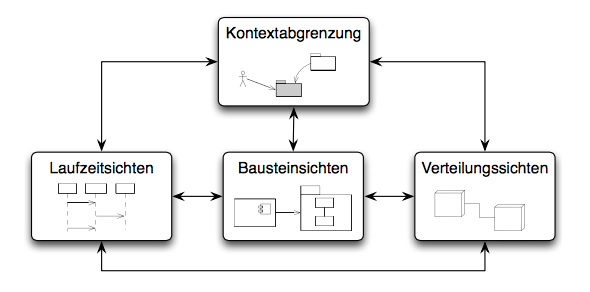
\includegraphics[width=0.9\textwidth]{../Bilder/sichten.png}
  }
  \caption{Vier Arten von Sichten (\cite{Starke201401})}

\end{figure}
\FloatBarrier



\textbf{Kontextsicht}\newline
Zeigt die Zusammenh�nge zwischen dem System und seinen Nachbarsystemen.\newline
\textbf{Bausteinsicht}\newline
Zeigt die statische Struktur, welche Bausteine Teil der Anwendung sind und welche
Beziehung sie zueinander haben.\newline
\textbf{Laufzeitsicht}\newline
Zeigt die Abl�ufe der Anwendung und die Zusammenarbeit der Bausteine zur Laufzeit.\newline
\textbf{Verteilungssicht}\newline
Zeigt, in welcher Umgebung das System abl�uft.

\section{Kontextabgrenzung}
Dieser Abschnitt stellt das Umfeld von der Applikation dar. Fu?r welche Benutzer ist es da, und mit welchen Fremdsystemen interagiert es?

\begin{center}
 \begin{minipage}{\linewidth}
	\centering
	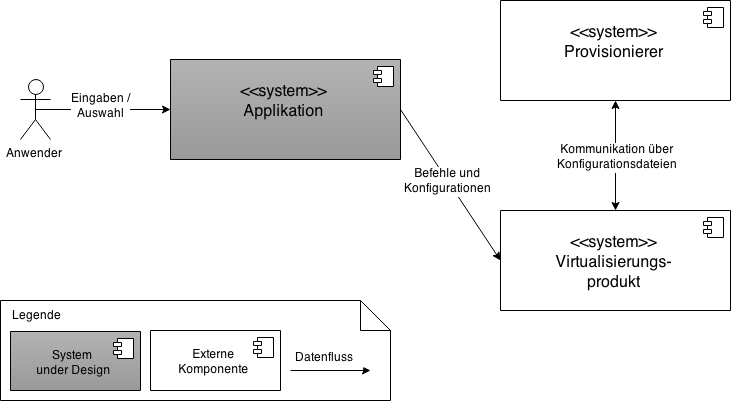
\includegraphics[scale=0.5]{../Bilder/kontextsicht.png}
	\captionof{figure}[kurze Bildunterschrift]{Bildunterschrift}
 \end{minipage}
\end{center}

In der dargestellten Kontextsicht, wird die d
\chapter{Sichten}
\section{Bausteinsicht}
\section{Laufzeitsicht}
\section{Verteilungssicht}
\section{Zusammenfassung}
